%%%%%%%%%%%%%%%%%%%%%%%%%%%%
% Master's Thesis          %	    										
% Fabian Burth, 2022-08-01 %
%%%%%%%%%%%%%%%%%%%%%%%%%%%%	

\npchapter{System Design}
This section describes the design of the \textit{Security and Compliance Data Lake}. It covers the conception of the data model, the selection of a database and the design of the API. Thereby, it especially discusses alternatives and focuses on giving detailed information about the ideas and motives that led to specific design decisions.

\section{Requirements}
Before actually going into the details of the systems design, the requirements have to be specified, since they are at the core of every design decision.  

\subsection{Functional Requirements}
The below table \ref{Tab:Requirements} provides a condensed list of the functional requirements for the Security and Compliance Data Lake. Thereby, every requirement is described by a short and precise but abstract statement of what functionality the system must have and an additional explanation which also includes an example. Additionally, there is a column categorizing the requirements as priority 1 or 2.\par 
Priority 1 is functionality deemed necessary for a central metadata store which should solve the limitations and problems identified in the previous chapters. Furthermore, priority 1 functionality is usually functionality that has to be considered in the design process and otherwise cannot be easily added without foundational remodeling.\par
Priority 2 functionality describes convenience features which are less urgent and may easily be added later on.
\begin{xltabular}{\linewidth}{|l|X|l|}
	\hline \hline \rowcolor{lightgray} \multicolumn{3}{ |l| } {\cellcolor{lightgray}{\textbf{Requirements}}}
	\\ \hline \rowcolor{lightgray}\textbf{Ref.\#} & \textbf{Functionality} & \textbf{Prio.}
	\\ \hline
	\endfirsthead
	
	\hline \hline \rowcolor{lightgray}\multicolumn{3}{|l|}{\cellcolor{lightgray}{\textbf{Requirements}}} \\ \hline \rowcolor{lightgray} \textbf{Ref.\#} & \textbf{Functionality} & \textbf{Prio.}\\ \hline
	\endhead
	
	\hline \multicolumn{3}{|r|}{{Continued on next page}} \\ \hline
	\endfoot
	
	\hline \caption{Requirements} \label{Tab:Requirements}
	\endlastfoot
	
	R.1 & The SCDL shall be able to consume and store metadata from multiple different data sources.\newline\newline
	The SCDL shall be able to work with any kind of metadata about software components.	Therefore, it has to be able to handle multiple different scanning tools as well as other kinds of data sources like build tools. As an example, it may have to consume data from BDBA, Mend but also Jenkins. Thus, it has to be considered that besides vulnerabilities and licenses, a variety of other metadata types may need to be added in the future. & 1\\
	\hline
	R.2 & The SCDL shall store the metadata from different data sources without aggregation\footnotemark{}.\newline\newline
	Different tools that generally serve the same purpose may provide similar information. As an example, BDBA and Mend are both SCA tools and therefore provide overlapping results. To ensure that no data is lost, this information shall not be combined and aggregated before storing.
	\footnotetext{\textit{aggregation} in this context means to merge the data about a package of e.g. a BDBA scan and a Mend scan to a single package entity instance} & 1\\
	\hline
	R.3 & The SCDL shall provide the metadata from different data sources with aggregation\footnotemark[\value{footnote}].\newline\newline
	As mentioned before, to ensure no data is lost, the data from different data sources shall be stored without aggregation. Anyway, to be consumed by a user, this data shall be aggregated. As an example, when querying all packages contained in a specific resource, the result returned by the SCDL shall not contain the same package twice in different representations, if it was identified by BDBA and by Mend. Instead, it shall contain an aggregated representation of the package. Thus, some kind of aggregation layer is needed which provides transparency regarding the data sources. & 1\\
	\hline
	R.4 & The SCDL shall provide a level of aggregation\footnotemark{} to group sources and resources.\newline\newline
	\footnotetext{\textit{aggregation} in this context refers to the "whole/part" semantic of the word \cite{UML}. Thus, since resources and sources are comprised of packages, they are both aggregations of packages. On a model level, the same applies for the relationships between packages and vulnerabilities or licenses as well as between entire deployments and the deployed resources.}
	As pointed out before, one problem also with SBOMs is the disconnection of the artifact metadata and the deployment information. To bridge this gap, an additional aggregation level for grouping artifacts is necessary. As an example, this additional aggregation level shall enable to group all resources contained in a specific deployment. & 1\\
	\hline
	R.5 & The SCDL shall enable users to query the metadata on different levels of aggregation\footnotemark[\value{footnote}]\newline\newline
	As an example, a user shall be able to query for all vulnerabilities in a specific resource, thus query on the aggregate level of resources. But a user shall also be able to query for all vulnerabilities in an entire specific deployment, thus querying on the aggregate level of deployments (querying on this level of aggregation enables to answer where Log4J is deployed). & 1\\
	\hline
	R.6 & The SCDL shall enable users to perform assessments.\newline\newline
	The relevance of specific pieces of information such as vulnerabilities or licenses depends on the usage context. As an example, while the internal usage of an altered OSS with a copyleft license is lawful, the distribution is not. Therefore, a possibility has to be provided to assess such pieces of information in the context of their occurrence. & 2\\
	\hline
	R.7 & The SCDL shall provide common data aggregation and filter functions for the queries.\newline\newline
	As an example, a user shall be able to filter for the vulnerability with the highest CVSS within a resource or shall be able to get the count of vulnerabilities within a resource. & 2\\
	\hline
	R.8 & The SCDL shall enable users to query the metadata in the common SBOM formats.\newline\newline
	In order to be able to fulfill governmental requirements of the executive order mentioned in the Software Bill of Materials section, the SCDL has to provide a way to to query the metadata in the common SBOM formats. As an example, a user shall be able to query the SPDX document for a specific resource. & 2\\
\end{xltabular}

So, by fulfilling this functional requirements, the Security and Compliance Data Lake may actually serve as a central application for storing and querying software metadata. Thereby, solving the problem of metadata being distributed throughout the development life cycle and bridging the gap between artifact metadata and deployment information.

\subsection{Non-functional Requirements}
Since this shall be a prototypical implementation, there is a strong focus on fulfilling the functional requirements. Thus, no concrete limits regarding performance or scalability such as a maximum response time of 5 seconds or support for up to 1000 concurrent users are set here. Considering the novelty of the topic, there is very few reference data and therefore, such specifications would be premature. However, for a central metadata store which may prospectively power dashboard web applications for monitoring purposes, scalability and performance definitely have to be considered in design decisions already.

\section{Data Model}
The basic entities relevant in the software supply chain are artifacts, thus sources and resources, and the packages comprising these artifacts. The definition of sources and resources is still the same as introduced in the previous chapter. Resources are capable of doing something and are usually executables or OCI Images. Sources are the code the resources are built from. Compliance scanners usually scan entire source code repositories or binaries. Through different methodologies, these tools detect the packages contained in these scanned artifacts on a best effort basis. In the context of this work, a package is defined as functional unit contained in artifacts, whereby it is usually a collection of files forming a library which is imported in the source code. By subsequently matching these packages against different databases such as the NVD, introduced in section \ref{sec:Vulnerability Management} "Vulnerability Management", known vulnerabilities and licenses are identified. To give a better idea of these results, figure \ref{fig:bdbaResult} in the appendix shows a snippet returned from the API of BDBA. The results on their own are useful already and provide interesting data about the above mentioned entities. But it is still loose metadata that lacks context information such as which deployments contain the corresponding entities. Therefore, an additional entity type to conduct further grouping is required. The OCM already introduced such an entity type, the component.\par
To conclude this, from a high level perspective, the important entities are \emph{components}, \emph{sources}, \emph{resources}, \emph{packages} and the information attached to these entities such as vulnerabilities and licenses. To generalize this and abstract away from specific data sources, the entity type representing these types of metadata is called \emph{info snippet}. So these entity types are the basic building blocks for the data model. From here on, it is getting rather complex and abstract. To still keep the explanations tangible, below figure \ref{fig:DataModel} already shows an \emph{entity-relationship model (ERM)} describing the final and universal data model. This may be used as a reference point throughout the following paragraphs, discussing the design decisions leading up to the specific entities, relationships and cardinalities.

\begin{figure}[H]
	\centering
	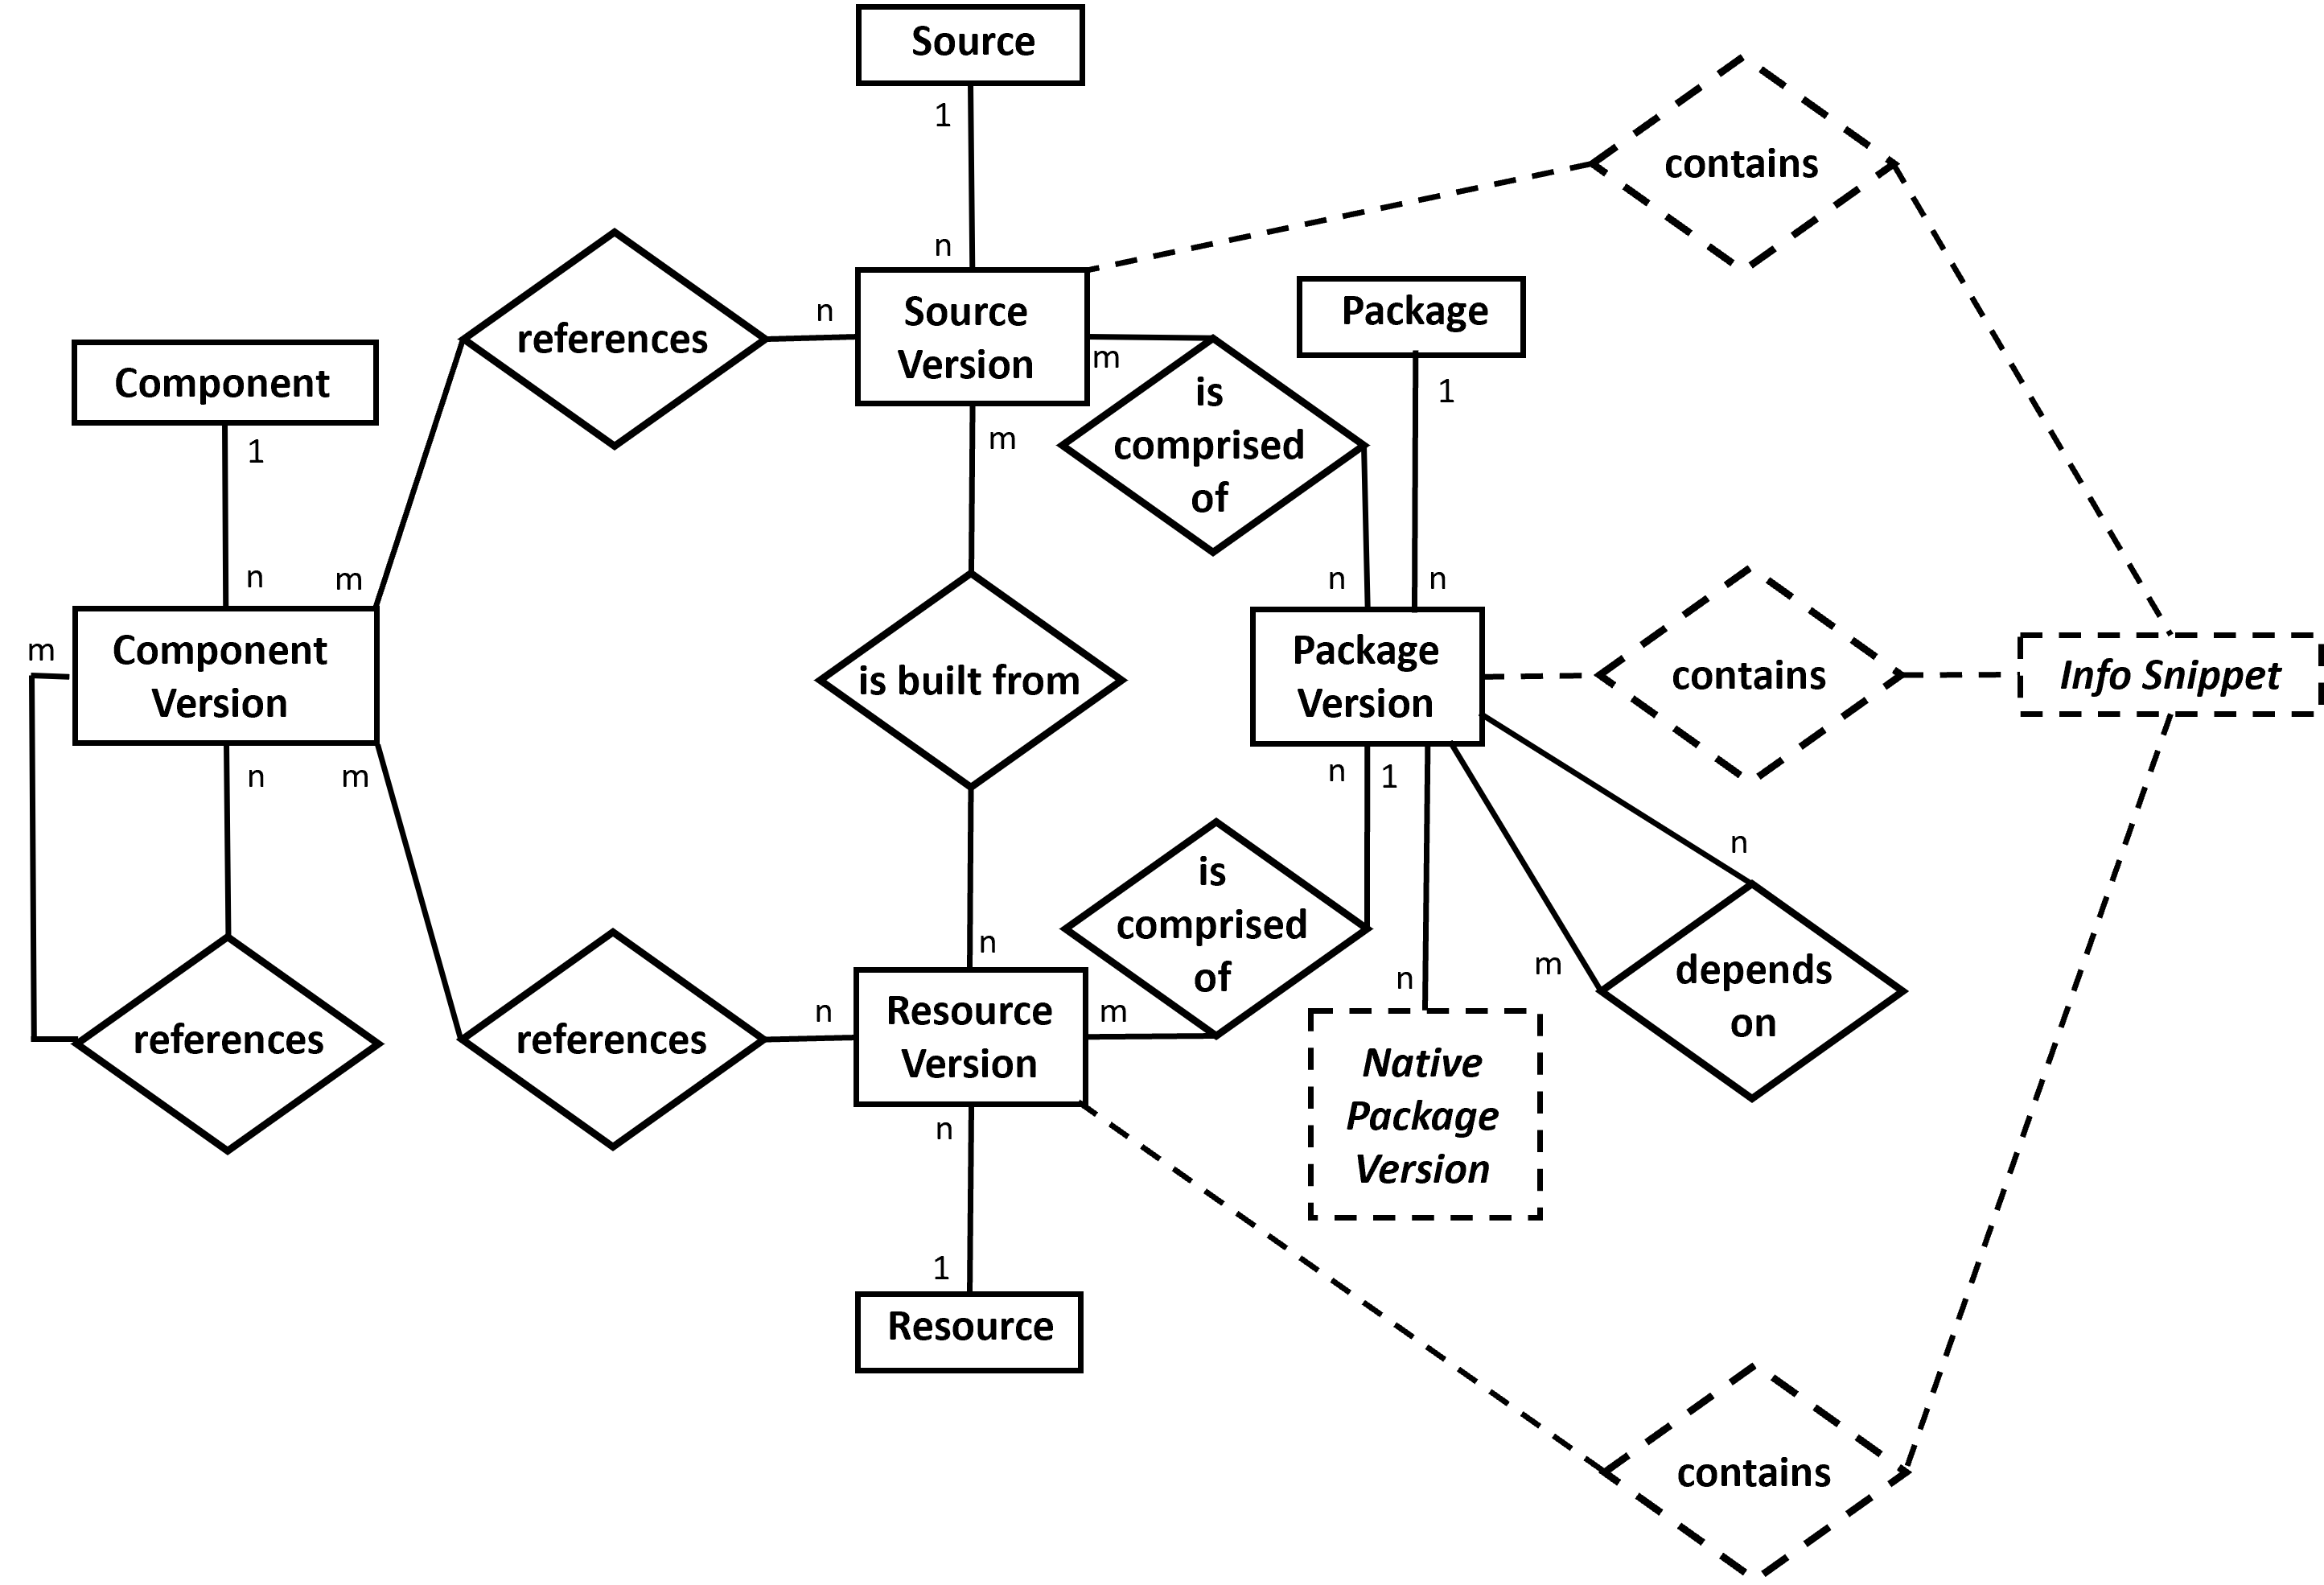
\includegraphics[scale=0.65]{datamodel}
	\caption[Data Model]{Data Model \source{Own Representation}}
	\label{fig:DataModel}
\end{figure} 

Even though the motivation behind every element may not be obvious immediately, the model as a whole should feel quite familiar and intuitive by now. An important notice at this point, the data model is inspired by the OCM. As mentioned above, especially the entity type \emph{component} is lend from the OCM. Since this thesis is written within SAP Gardener, a seamless integration of the this Security and Compliance Data Lake such as described in the previous chapter is of course also a requirement, even though it is not explicit listed. But still, the Security and Compliance Data Lake is designed independent of the OCM. Thus, in theory it is entirely possible to use a different kind of component model. As an example, if one is able to express the concept of \emph{components} and \emph{artifacts} with the means of the SPDX standard, one could use SPDX instead of OCM to provide this structural information. Or, since SPDX is not optimal for this purpose, one could create and use an own component model, as long as it has the means to express \emph{components} and \emph{artifacts} (There is generally no necessity to distinct between \emph{sources} and \emph{resources}. \emph{Sources} could be treated as \emph{resources}, at the only cost of losing the connecting "is built from"-information between the two entities.).

\subsection{Universal Data Model}
Contrary to common ERMs, the one in figure \ref{fig:DataModel} does not have any properties. There are two major reasons for this. Firstly, the just mentioned independence of a specific component model would hardly be possible if the data model would define fixed predefined properties for each entity type. Secondly, the different scanning tools provide a wide range of information about packages and other data sources but scanning tools may also be added. It is therefore practically impossible to foresee what properties may be needed. Besides, these may vary depending on the user of the Security and Compliance Data Lake.\par
Another special feature of above ERM are the entity types and relationships illustrated with dash lines. These represent classes of entity types and relationships. Since the whole set of data sources cannot be known upfront, the whole set of potentially required \emph{Info Snippets} cannot as well. As already mentioned in several examples before, when adding a build tool as data source, an entity type \emph{Build Information} may be needed. Also, the relationships of different \emph{Info Snippet} entity types may vary. While a \emph{Vulnerability} and a \emph{License} is usually \emph{contained} in multiple \emph{Package Versions} leading to a (n:m)-relationship, a \emph{Build Information} is usually associated to one \emph{Resource Version} leading to a (1:n)-relationship. But generally, \emph{Info Snippets} could be associated to any other entity type in the data model with any cardinality. This kind of flexibility is necessary to enable R.1 (consume and store metadata from multiple different data sources). The \emph{Native Package Version} correspondingly illustrates the representation of a package, native to a concrete data source. Thus, instances of \emph{Native Package Versions} may be \emph{BDBA Package}, \emph{Mend Package} or even \emph{Jenkins Package}. So if all three data sources provide information about the exact same \emph{Package Version}, each representation may be stored without a need to merge their properties before storing. Thereby, this enables R.2 (store metadata from different data sources without aggregation). Then, a set of properties commonly provided by all of the data sources may be aggregated on \emph{Package Version} level, thereby also enabling R.5 (provide the metadata from different data sources with aggregation). So, all these \emph{Native Package Versions} representing the exact same package are related to the same \emph{Package Version} on the model level. As the different data sources may use different identifiers for the packages, the merging process cannot be triggered automatically. Hence, until a human defines that the \emph{BDBA Package}, the \emph{Mend Package} and the \emph{Jenkins Package} are actually representations of the same package, no merging is done and each is related to a different \emph{Package Version}.\\\par
So after explaining the special features of above ERM, the common entity types and relationships may be discussed. The basic entity type \emph{component} is broken down into two distinct entity types, \emph{Component} and \emph{Component Version}. As immediately noticeable, this distinction is done for each of the basic entity types. \emph{Component} is a purely abstract entity type. It merely groups all the versions of the same component together. Thereby, the \emph{Component} may provide information about the semantics of this grouping such as whether this \emph{Component} describes a specific deployment or whether it describes all software used by a department. Thus, information that is identical for all versions of this component and would have to be stored redundantly for each \emph{Component Version} otherwise. Naturally, there are multiple \emph{Component Versions} of each \emph{Component}. Therefore, the (1:n)-cardinality here is self-explaining.\par 
As established by the previously described grouping semantic of \emph{components}, a \emph{Component Version} may reference multiple other \emph{Component Versions}. For example, a \emph{Component Version} describing a specific version of a deployment may reference multiple other \emph{Component Versions} such as \emph{Component Versions} describing specific versions of a web server, a service and a database. Reciprocal, a \emph{Component Version} may of course be referenced by multiple \emph{Component Versions}. For example, a \emph{Component Version} describing a web server may be referenced by several \emph{Component Versions} describing different versions of the same deployment or entirely different deployments. Thus, this is a recursive (n:m)-relationship. There may also be a need to store additional occurrence specific metadata as properties of the \emph{references}. Considering the above example, such occurrence specific metadata may provide information about the usage of the web server within the deployment, hence whether it is used as a HTTP server or as a load balancer. Together, these model elements fulfill requirement R.4 (provide an aggregation level to group sources and resources).\par
Furthermore, a \emph{Component Version} may also reference multiple \emph{Source Versions} and \emph{Resource Versions}. As an example, the \emph{Resource Versions} comprising the web server and the \emph{Source Versions} from which the respective \emph{Resource Versions} were built. As before, with the recursive relationship of \emph{Component Versions}, the \emph{Source Versions} and \emph{Resource Versions} may of course also be referenced by multiple \emph{Component Versions}, resulting in a (n:m)-relationship. Again, there may be a need to store additional occurrence specific metadata as properties of the \emph{references}. Specifically, these \emph{references} may be used to store \emph{triage} information. As this \emph{reference} describes the usage context of the \emph{Artifact}, one may for example decide whether a copyleft license is or is not acceptable here. The relationship between \emph{Source} and \emph{Source Version} as well as between \emph{Resource} and \emph{Resource Version} is similar to the relationship between \emph{Component} and \emph{Component Versions}. But the abstract \emph{Source} and \emph{Resource} entity types actually do have a concrete purpose but only preventing redundant storage of certain properties. In this case, these abstract entities may have properties to store \emph{triage policies}. As an example, one may store that a specific vulnerability may be ignored for the usage of \emph{Resource Versions} v1.0.0 to v1.2.3 of a respective \emph{Resource} within \emph{Component Versions} v1.4.2 to v1.4.12 of a specific \emph{Component}. The \emph{references} and the abstract \emph{Source} and \emph{Resource} entities thereby enable the fulfillment of requirement R.6 (enable users to perform assessments).\par 
\emph{Resource Versions} may also reference the \emph{Source Versions} they are built from. A \emph{Resource Version} may be built from multiple \emph{Source Versions} and a \emph{Source Version} may be used to build multiple \emph{Resource Versions}. This also results in a (n:m)-relationship.\par
Since \emph{Artifacts} are comprised of \emph{Package Versions} and the same \emph{Package Version} may occur in multiple \emph{Artifacts}, both \emph{Source Version} as well as \emph{Resource Version} have a (n:m)-relationship to \emph{Package Version}. Again, there may be a need to store additional occurrence specific metadata as properties of the \emph{is comprised of} relationship.\par
The relationship between \emph{Package} and \emph{Package Version} is again similar to the relationship between \emph{Component} and \emph{Component Versions}. But as already explained \emph{packages} are broken down even further into three different entity types and thereby three aggregate levels. Since several data sources may provide different representations, thus different \emph{Native Package Versions}, of the same \emph{Package Version}, the cardinality of this relationship is (1:n). \emph{Package Versions} frequently \emph{depend on} other \emph{Package Versions} and so on. This may lead to quite long chains of dependencies. This has to be kept in mind as these transitive dependencies are also relevant when trying to answer the question, whether a certain \emph{Artifact} or \emph{Component} contains a specific \emph{Package} such as Log4J, and its corresponding vulnerabilities.\par
Finally there is the \emph{Info Snippet} class of entity types. As explained above, different \emph{Info Snippet} entity types may have relationships to different entity types with different cardinalities.

\subsection{Insights into the Development Process}
At this point, some insight into the development process may be beneficial to understand this design decisions. The scope of this central data store was initially much narrower. The first PoC was actually strictly bound to the OCM. Therefore, the data model predefined the properties of \emph{component} and \emph{artifact} entity types. As it was bound to the OCM, there was no issue in doing so. But the data model also predefined the properties of the \emph{package} entity types. In fact, the third aggregate level for \emph{packages}, \emph{Native Package Version} did not exist at all. Instead, the \emph{Package Version} entity type had a set of properties that was hoped to be common and harmonizable throughout all prospective data sources. At this time, the application was also tailored to only having scanning tools as data sources. Therefore, to define this set of properties, the API documentations of different scanning tools were analyzed for the common and most important properties, especially the ones of BDBA and Mend \cite{MendAPI}. Additionally, to get a better understanding, both scanners were used on some artifacts to get some sample data. Then, the provided attributes were narrowed down and some interviews with developers were conducted. A huge effort was made here, as this was such an important decision. Also, instead of having the \emph{Info Snippet} class of entity types, there was only a \emph{Vulnerability} and a \emph{License} entity type whose set of properties was defined in the same process. Besides the fact that there was already a substantial amount of disagreement between different developers which properties were actually required, by the time the PoC was finished, several new use cases were discovered that required additional properties and even entire additional entities to provide other information than about vulnerabilities or licenses.\par
This led to a change in perspective, interpreting the task of defining the right entity types with the right properties rather as a task to make the entire application extensible regarding the respective entity types and properties. But this flexibility and extensibility comes at the cost of a highly increased overall complexity. Apart from remodeling the data model, it also required a completely new architecture and completely different implementation. Thus, only after that, the scope widened drastically, also allowing other component models. Consequently, as a kind of disclaimer, the design process presented here is not exactly as chronological as it may initially seem, since it hides a complete development iteration leading up to the final concepts.

\subsection{Application of the Data Model}
Although a great effort was made to make the data model as tangible as possible, it may still be hard to grasp due to its abstract nature, omitting properties and introducing classes of entity types. Therefore, this section discusses how this data model could be applied. As reference component model, the OCM is used and as reference data sources, only BDBA is used. This thereby also reveals a problem that has to be faced when applying this data model to a real world use case. The figure \ref{fig:RefDataModel} below shows the corresponding data model instance.\par

\begin{figure}[H]
	\centering
	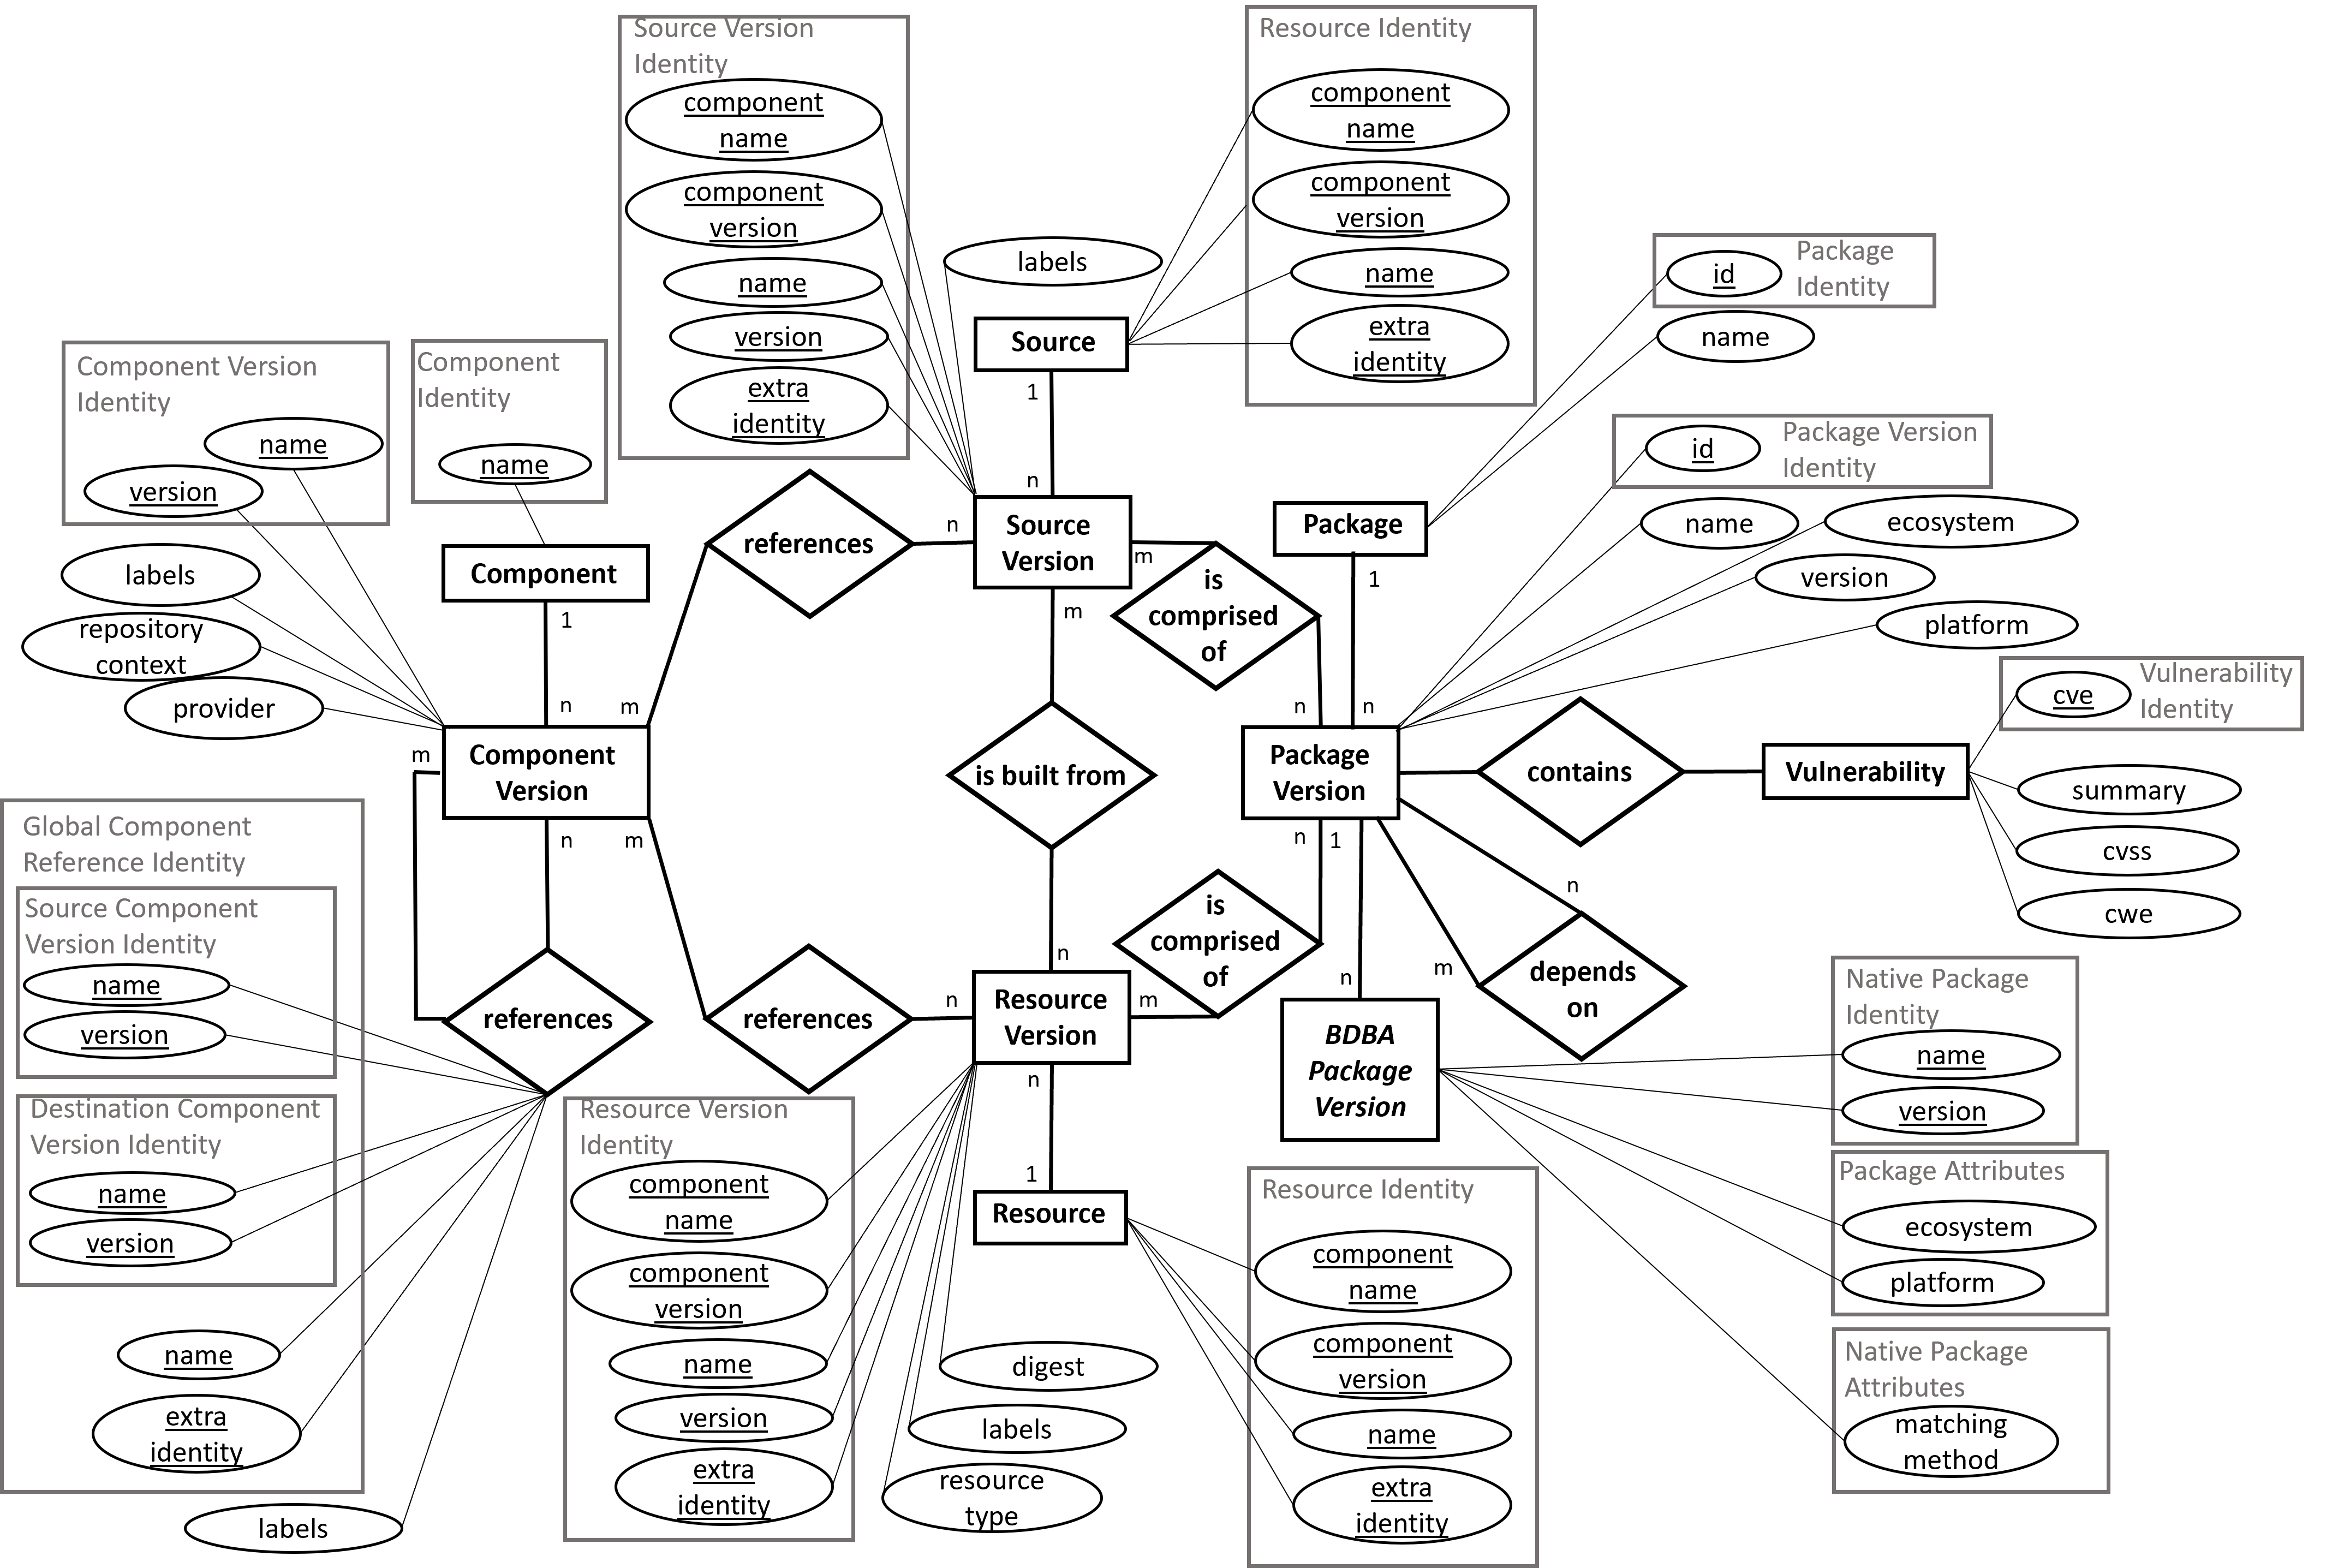
\includegraphics[scale=0.45]{refdatamodel}
	\caption[Data Model]{Example Data Model Instance \source{Own Representation}}
	\label{fig:RefDataModel}
\end{figure}

The figure is very crowded. But this is necessary, as the purpose of this figure is to provide a concrete and thorough example of how the abstract universal data model may be applied to specific component models and tools.\par
The important aspect to point out here is the relationship between \emph{Component Version} and \emph{Source Version} and between \emph{Component Version} and \emph{Resource Version}. Although depicted as a relationship with (n:m)-cardinatility in compliance with the universal data model, due to the \emph{Component Version-Local Identity} of \emph{Source Version} and \emph{Resource Version}, these can actually only be (1:n)-relationships. There were detailed explanations about this in section \ref{sec:Open Component Model} "Open Component Model". \emph{Source Version} and \emph{Resource Version} were referred to as \emph{Source Reference} and \emph{Resource Reference} because in the context of OCM, instead of actually representing the technical artifact, they only reference the technical artifact through their \emph{access} property. The SAP Gardener team chose this initially rather confusing specification of \emph{Source Versions} and \emph{Resource Versions} with \emph{Local Identities} since in practice, it is difficult to reliably determine whether two referenced technical artifacts are actually the same technical artifact.\par 
The following sections further explain the issue and discuss different approaches of dealing with this artifact identity problem. They thereby point out the use cases and limitations of each approach. The terms \emph{Resource Version} and \emph{Source Version} are from here on used as in the context of OCM, thus these terms are interchangeable with \emph{Resource Reference} and \emph{Source Reference}. 

\subsubsection{Uniform Resource Identifiers} 
The initial and most obvious approach is to treat technical artifacts just as components. Thus, assign a globally unique name and a version to each technical artifact. But the reason this works for components is that these are purely abstract or logical entities. Thus, there is no digital or rather technical twin such as source code or a binary that corresponds to a specific component. If there is, who guarantees that two \emph{Resource Versions} with the same name and the same version actually point to the same binary? Or reciprocal, that two \emph{Resource Versions} pointing to the same binary actually have the same name and version? Where and how would one look up this globally unique name of a \emph{Resource Version} in the first place?\par
A common approach in this situations are URIs. As introduced in section \ref{sec:Software Identification} "Software Identification", by providing a specification of how this URI is composed, standards such as purl provide a way to create theoretically reproducible identifiers. Theoretically, because in practice composing this URIs still has to be done by people. Consequently, there is always room for interpretation and human error. Imagine a \emph{Resource Version} in two different \emph{Component Versions} referencing artifacts in two different repositories, for example \lstinline|github.com/example/nginx| with tag \lstinline|1.0.3| and \lstinline|github.com/example/nginx-webserver| also with tag \lstinline|1.0.3|. At this point, it is difficult to determine, whether these are technically the same artifact and should consequently have the same URI. Thus, this approach is unreliable and impractical.

\subsubsection{Content-Addressable Uniform Resource Identifiers}
In order to guarantee that two \emph{Resource Versions} with the same URI actually point to the same binary and that two \emph{Resource Versions} pointing to the same binary actually have the same URI, this URI has to be content-addressable. Therefore, a coupling of identity and location is necessary.\par 
The straight forward approach to do this in practice is to use the URLs provided by the repositories. But as the example above shows, this approach is not really flexible, as the URLs have to be immutable.\par 
The OCM specifies that the access property is variable. Still in section \ref{sec:Development and Deployment Landscape at SAP Gardener} "Development and Deployment Landscape at SAP Gardener", it is explained that images, thus technical artifacts, and component descriptors are copied from the development landscape into other landscapes and that the access property changes in this process. So the development landscape may serve as single source of truth and the respective artifact URLs of the access property may be used as this content-addressable URI. Even though the URLs in the access property of the component descriptors in other landscapes may differ from the URI globally identifying the artifact, as this URI is used to copy the artifact to the location referenced by the URL in the new access property, it is the same per construction. So this approach is generally reliable and practical.\par
SAP Gardener did not consider this approach anyway, as it is more complex and globally unique identifiers for artifacts were not relevant for the original scope of the OCM, which was deployment automation. 

\subsubsection{Digests as Global Identifiers} 
So, another option to determine whether two artifacts are technically the same, even though they are located in different repositories is through calculating a suitable \emph{normalized digest}.\par 
A \emph{digest} refers to a short, fixed-length string calculated through a hash function \cite{Cryptography}. There are several features in which artifacts may vary but that are irrelevant for their comparison. For example, the exact same source code file may provide different digests when hashed with the exact same hash method, depending on whether it is hashed on a windows or a linux machine. This is due to the different line endings, thus "Carriage Return and Line Feed" on windows and "Line Feed" on linux. In order to calculate a normalized digest, the input data for the hash function is prepared so that such irrelevant features do not have an impact on the digest. So the input data is normalized.\par
This approach is generally reliable and clean, but there are again several problems. When looking at figure \ref{fig:RefDataModel} above, there is already a digest property available for \emph{Resource Versions}. As described in section \ref{sec:Open Component Model} "Open Component Model", this digest property specifies a hash function, a normalization function and the corresponding digest value. Although the primary reason for this is that different kinds of resources, for example executeables and OCI Images, may need different kinds of normalization functions, this also means that the same artifact may have different digest values in different \emph{Component Versions}.\par
Consequently, the digests need to be calculated in a standardized way, independent of the OCM. But even then, there is still another issue regarding the data model. There is no way to decide whether artifacts with different normalized digests may be different versions of the same artifact. Thus, the additional aggregate level, \emph{Source} and \emph{Resource}, required for triage policies is practically impossible to determine.

\subsubsection{Local Identifiers}
This is the approach used in the OCM. This concept was explained in detail in section \ref{sec:Open Component Model} "Open Component Model". The detailed examination of the general artifact identity problem also showed implicitly why differentiating between the terms \emph{Resource}, \emph{Resource Version} or \emph{Source}, \emph{Source Version} and \emph{Resource Reference} and \emph{Source Reference} is so difficult from a modeling perspective.\par
After all, the most important aspect to point out here, is that although it is not intuitive, only having local identifiers for artifacts is still quite functional regarding the goals which shall be achieved by the data model.

\begin{figure}[H]
	\centering
	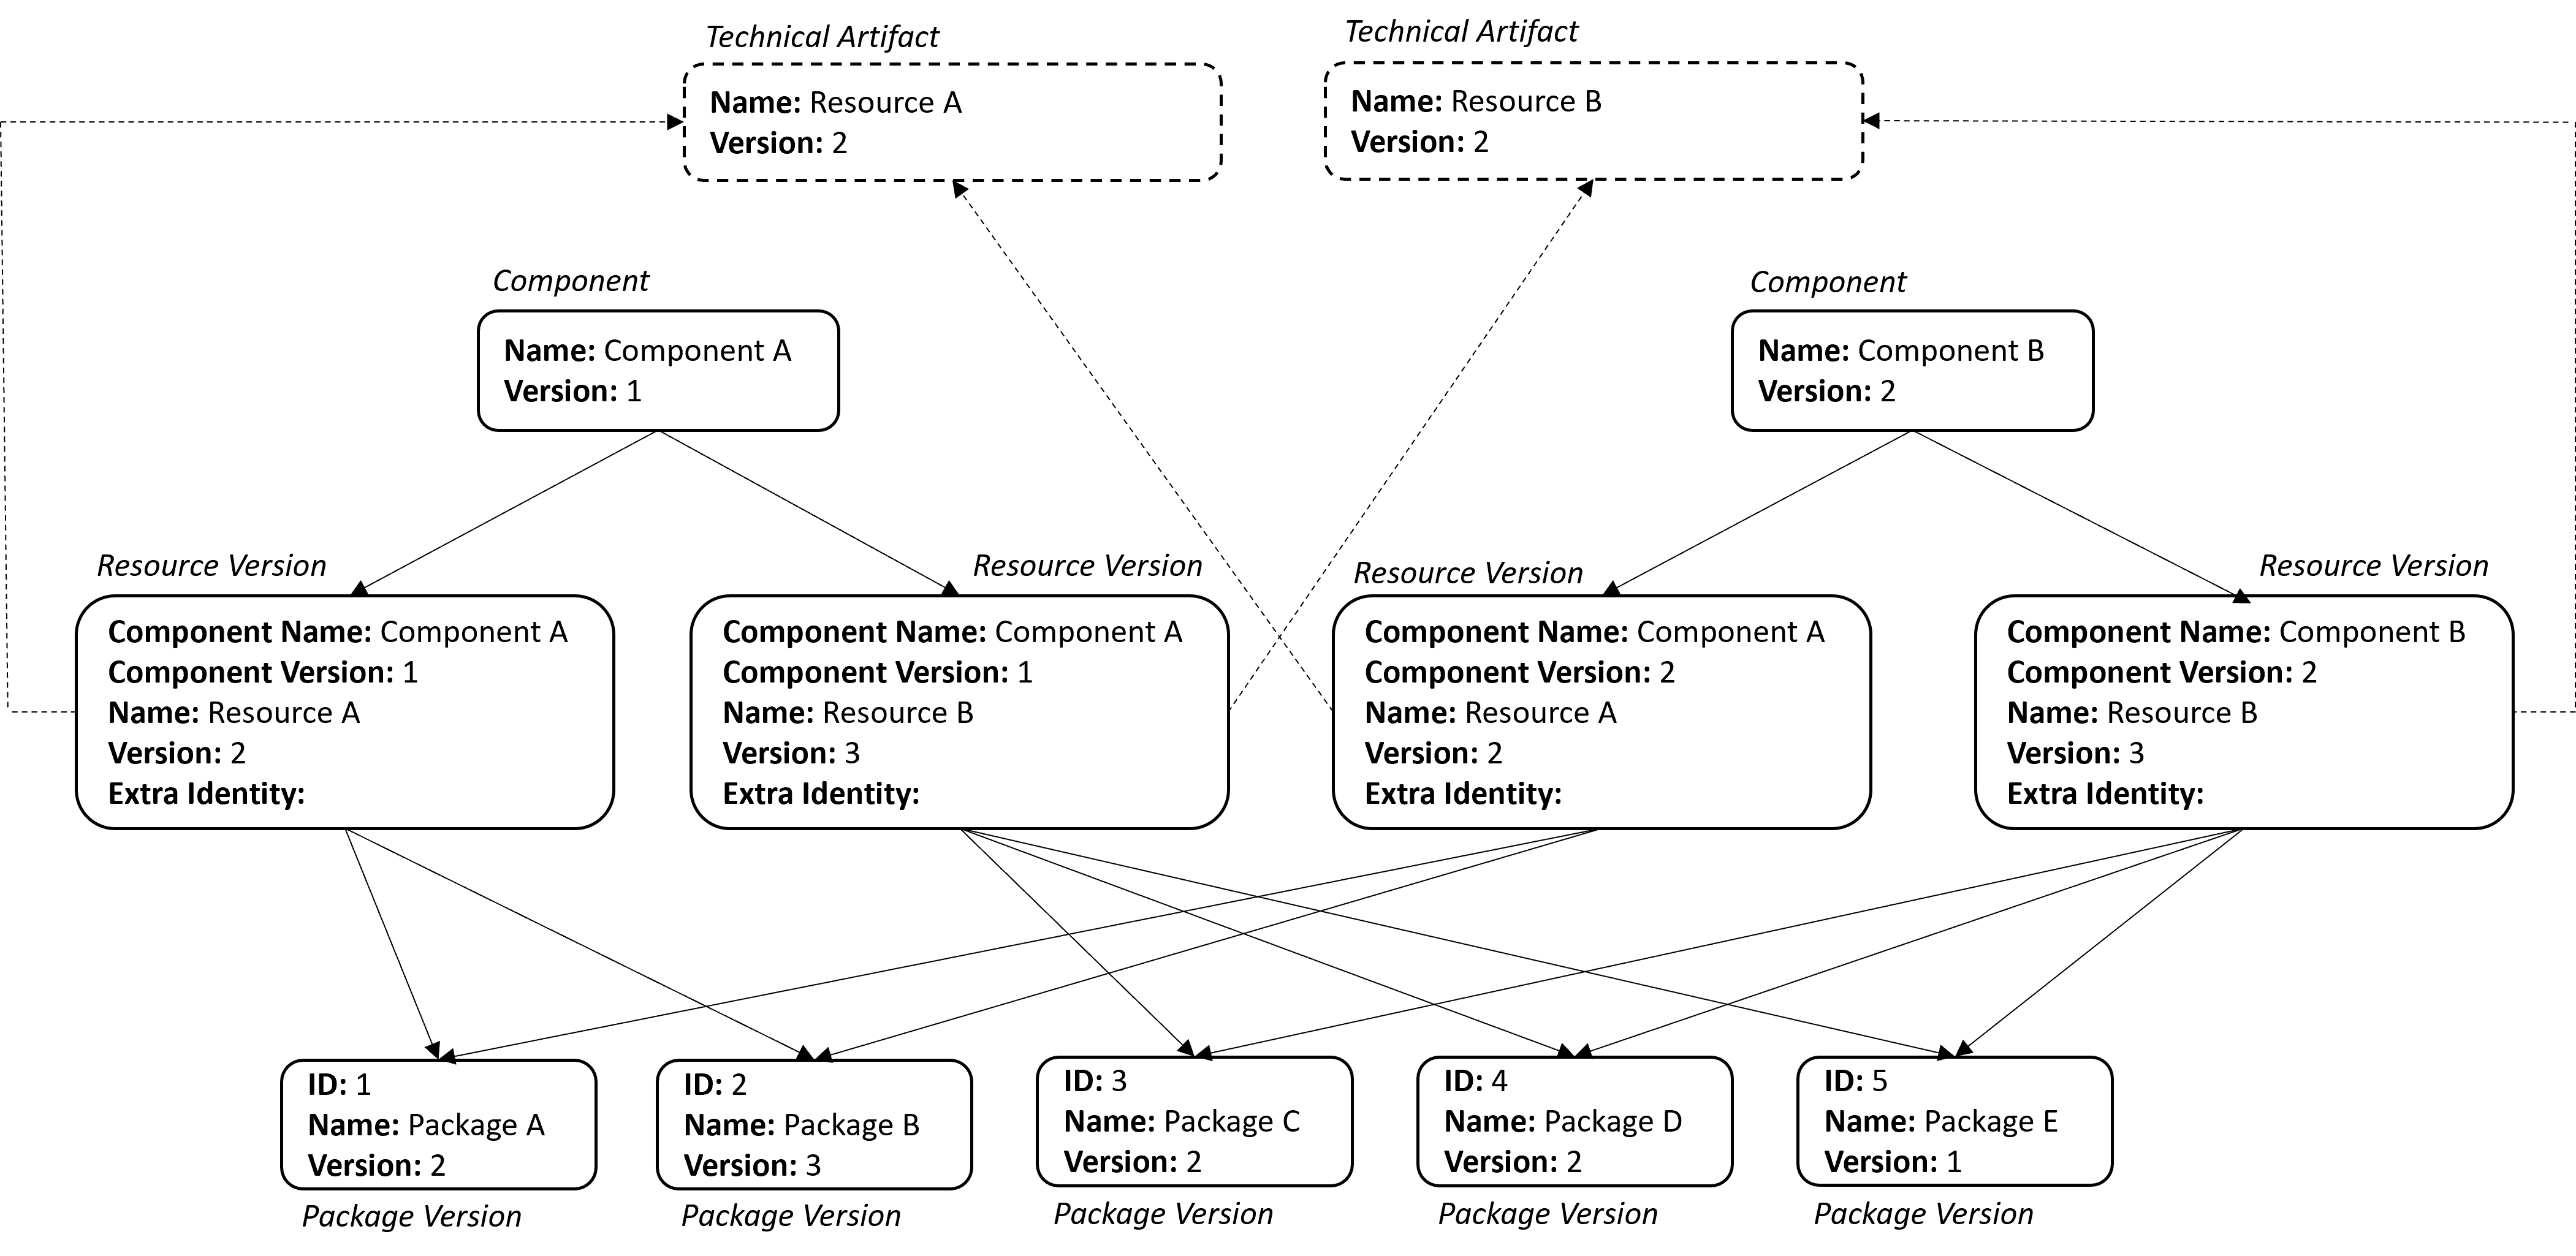
\includegraphics[scale=0.45]{localartifactidentity}
	\caption[Data Model]{Local Artifact Identities \source{Own Representation}}
	\label{fig:LocalArtifactIdentity}
\end{figure}

Figure \ref{fig:LocalArtifactIdentity} shows two components that reference the exact same technical artifacts. But since the \emph{Identity} of \emph{Resource Versions} is local, the component name and version are part of the \emph{Resource Versions Identity}, as also shown in figure \ref{fig:RefDataModel}. Thus, it appears as they are referencing different artifacts. But as the packages comprising the \emph{Resource Versions} are identified by scanning the technical artifact accessed through the access property, they are the same for the \emph{Resource Versions} which practically reference the same technical artifact.\par 
So, for answering questions such as which deployment contains Log4J and its corresponding vulnerabilities, the local artifact identities do not make a difference. As in practice, it may also be assumed that within a \emph{Component}, \emph{Resource Versions} with the same name but different version numbers are in fact pointing to different versions of the same technical artifact, the \emph{Resource} aggregate level is also kind of possible. But its scope and the scope of \emph{triage policies} within these entities respectively is of course limited to a certain \emph{Component}. Furthermore, attaching \emph{Build Information} and other \emph{Info Snippets} to artifacts is difficult with this approach.


\section{Database}
After the application context and data model are defined, a suitable database has to be selected. Therefore, this section analyzes the most relevant database technologies regarding their applicability as a central data store based on the previously defined data model.


\subsection{Relational Databases}
The first database technology analyzed are relational databases. They are by far the most popular and widely used database technology. This is represented in Stack Overflow's 2021 developer survey \cite{StackoverflowDeveloperSurvey}. Among the technologies discussed in detail here, it has also been around for the longest as the original paper introducing the relational model for databases by Edgar Codd was published in 1970 \cite{RelationalDatabaseOriginalPaper}. Therefore, the technology itself is very mature. everybody has know how. worth considering for every enterprise project.\par
A quick repetition of the foundations of relational databases. The name "relational database" stems from the mathematical definition of relation. Thus, given sets 
\subsection{Document Store Databases}
\subsection{Graph Databases}


\section{API}

